\documentclass[brudnopis]{xmgr}

%\defaultfontfeatures{Scale=MatchLowercase}
%\setmainfont[Numbers=OldStyle,Ligatures=TeX]{Minion Pro}
%\setsansfont[Numbers=OldStyle,Ligatures=TeX]{Myriad Pro}
% for fontspec version < 2.0
\setmainfont[Numbers=OldStyle,Mapping=tex-text]{Minion Pro}
\setsansfont[Numbers=OldStyle,Mapping=tex-text]{Myriad Pro}
%\setmonofont[Scale=0.75]{Monaco}
\usepackage{hyperref}
\usepackage{enumerate}
\usepackage{minted}
\usepackage{caption}
% Opcjonalnie identyfikator dokumentu
% drukowany tylko z włączoną opcją 'brudnopis':
\wersja   {wersja wstępna [\ymdtoday]}

\author   {Oskar Plichta}
\nralbumu {195009}
\email    {oskar.plichta22@gmail.com}


\title    {Budowa aplikacji modularnej do udostępniania fotografii  w web 3.0}
\date     {2015}
\miejsce  {Gdańsk}

\opiekun  {dr W. Bzyl}

% dodatkowe polecenia
%\renewcommand{\filename}[1]{\texttt{#1}}

\begin{document}

\begin{abstract}
W pracy zostanie przedstawiony program do udostępniania fotografii na kilka serwisów społecznościowych jednocześnie z intuicyjnym interfejsem Material Design. Dzięki temu w prosty i szybki sposób można podzielić się swoimi zdjęciami z innymi użytkownikami kilku sieci społecznościowych. Aplikacja będzie wykonana z dwóch modułów - części serwerowej i wizualnej. Część serwerowa jest oparta o \textit{Ruby on Rails} a wizualna wykonana w \textit{EmberJS} oraz \textit{Materialize}. Aplikacje mobilna dla systemu Android wykonane zostały dzięki aplikacji \textit{Cordova}, która pozwala przekształcić aplikację opartą o \textit{EmberJS} oraz \textit{Ember CLI} w natywną aplikacje dla danego systemu mobilnego. Ostatecznie aplikacja została wykonana zgodnie z założeniami i spełnia wyznaczone cele.

\end{abstract}
\keywords{\textit{User Interface, Material Design, Ruby on Rails, EmberJS, PostgreSQL, RSpec, QUnit}}

% tytuł i spis treści
\maketitle
%
% wstęp
\introduction
\indent Fotografie są jednym z najczęstszych typów danych przesyłanych w Web 3.0. Gwałtowny rozrost sieci społecznościowych spowodował, że prawie każdy udostępnia zdjęcia aby podzielić się nimi z rodziną i przyjaciółmi. Temat wysyłania zdjęć do kilku serwisów jednocześnie, tak aby nie jeszcze raz nie powtarzać tej samej czynności na innym serwisie społecznościowym, pozostaje otwarty i dlatego postanowiłem go zgłębić.
\newline\indent Portale takie jak Facebook, Flickr czy Twitter prześcigają się w tym aby wysyłanie zdjęć na ich serwer było jak najprostsze. Większość z nich pozwala na tzw. \textit{drag and drop}\footnote{ang. \textit{drag and drop} - przeciągnij i upuść} fotografii oraz na wysyłanie ich do innych serwisów. Zakładając, że mamy zdjęcia z wakacji i chcemy je udostępnić na Facebooku oraz umieścić na naszym koncie Flickr w celu archiwizacji musimy zalogować się na Facebooka, następnie wysłać zdjęcia na serwer Facebooka, ewentualnie dopisać opis i kliknąć w przycisk do udostępniania, po czym całość powtórzyć na serwisie Flickr.Aplikacja, którą opisuje w tej pracy pozwala na jednoczesne wysyłanie zdjęć na kilka serwisów społecznościowych za pomocą kilku kliknięć. Wystarczy wybrać zdjęcia dzięki drag and drop, zalogować się na wybrane przez nas serwisy a następnie kliknąć wyślij. Wszystko przebiega szybko i sprawnie a my oszczędzamy nasz czas.  Aplikacja ta jest tzw. aplikacją modułową co znaczy, że w przeciwieństwie do aplikacji monolitycznej, składa się z  niezależnych od siebie części tj. serwerowej oraz wizualnej. Obie części komunikują się ze sobą za pomocą wiadomości JSON. Część serwerowa odpowiada za komunikację z bazą danych, komunikację z serwerami zewnętrznymi oraz autoryzację użytkowników i wysyłanie danych do front-endu czyli aplikacji wizualnej. Zostanie ona wykonana w języku Ruby i frameworku \textit{Ruby on Rails}.   Aplikacja wizualna, która zostanie wykonana w języku JavaScript i frameworku \textit{EmberJS}, ma za zadanie wyświetlanie danych w przystępnej formie dla użytkownika poprzez tzw. interfejs. Omówię zagadnienie aplikacji modularnej i monolitycznej bardziej szczegółowo w jednym z kolejnych rozdziałów. Interfejs użytkownika \footnote{ang. \textit{User Interface} - UI}  jest podstawowym sposobem komunikacji pomiędzy człowiekiem a maszyną dlatego tak ważne jest, aby był on intuicyjny i przyjazny dla użytkownika. Postaram się pokazać dlaczego UI w mojej aplikacji jest przyjazny, intuicyjny dla użytkownika i pozwala mu na wydajną pracę a wszystko dzięki wytycznym Google Material Design, które jest nowym designem dla aplikacji od firmy Google. Więcej na temat Material Design oraz interfejsu aplikacji PicDrop w kolejnych rozdziałach.\newline \indent Większość smartphonów posiada dobrej jakości aparaty, zarówno z przodu jak i z tyłu urządzenia, dlatego w każdej chwili możemy wysłać zdjęcia z dowolnego miejsca do rodziny i przyjaciół poprzez sieci społecznościowe, za pomocą natywnej aplikacji na dany system mobilny. Dzięki temu, że moja aplikacja jest modułowa, jej część serwerowa czyli API pozwala na połączenie z nią różnych części wizualnych tzw. front-end z systemów mobilnych takich jak np. iOS lub Android. Jest to możliwe dzięki aplikacji Cordova, która zamienia aplikację \textit{EmberJS} w natywną aplikację na dany system mobilny przez co jest ona łatwiejsza w obsłudze i lepiej wykorzystuje mały wyświetlacz smartphona niż aplikacja przeglądarkowa. Opiszę dokładniej ten proces w odpowiednim rozdziale oraz podam inne zalety aplikacji natywnej. Wskażę również z jakimi problemami musi się uporać \textit{developer} aplikacji webowych, aby jego aplikacja była intuicyjna i funkcjonalna. Wyjaśnię, które elementy mojej aplikacji testuję i w jaki sposób. Opierając się na  doświadczeniach innych badaczy  między innymi Roberta Hoekmana jr  \cite {magiaUI} oraz Jenifer Tidwell  \cite {projektowanieUI}, którzy opisali swoje spostrzeżenia w ich książkach, postaram się napisać aplikacje PicDrop, która  będzie miała przyjazne UI i pozwoli na łatwe udostępnianie treści. Opiszę dlaczego wybrałem \textit{EmberJS}, \textit{MaterializeCSS} oraz \textit{Ruby on Rails} do stworzenia tej aplikacji i dlaczego te technologie uważam za najlepszy wybór.


\chapter{Budowa aplikacji modularnej do udostępniania fotografii  w web 3.0}

\section{Porównanie dostępnych rozwiązań}
Każdy serwis społecznościowy posiada swoje możliwości udostępniania zdjęć, które ograniczają się do jednego serwisu. Tak więc jeśli chcemy wgrać swoje zdjęcia jednocześnie na Facebooka, żeby zobaczyli je nasi znajomi oraz Flickr w celu archiwizacji to musimy je wgrać na jeden z tych dwóch serwisów a następnie na kolejny. Takie rozwiązanie zajmuje dużo czasu i jest niekorzystne dla użytkownika. Serwis Facebook, który jest najpopularniejszym serwisem społecznościowym, zrzesza ponad 500 milionów użytkowników. Udostępnianie zdjęć poprzez ten serwis polega na kliknięciu w ikonkę zdjęcia i wybraniu danego pliku, bądź przeciągnięciu i upuszczeniu pliku w odpowiednim miejscu. Możemy dopisać, krótki tekst i po naciśnięciu guzika wyślij, post pojawi się na naszej tablicy. Facebook nie pozwala na udostępnianie zdjęć poza swoją stroną, także jeżeli mamy znajomych nie posiadających konta na tym serwisie to nie zobaczą oni naszych zdjęć. \newline \indent \textit{Flickr} jest serwisem dla miłośników fotografii, który daje nam, aż 1 TB na przechowywanie naszych zdjęć. Pozwala on również na udostępnianie plików także do innych serwisów społecznościowych. Umieszczanie zdjęć w tym serwisie jest podobne do rozwiązania stosowanego w Facebooku, to znaczy albo wybieramy pliki albo przeciągamy je do okna przeglądarki. Po wgraniu ich na serwer możemy je udostępnić dalej poprzez wybranie zdjęć. Aktualnie nie ma serwisu, który by pozwalał na wysyłanie zdjęć do dwóch serwisów jednocześnie. Z tego powodu postanowiłem stworzyć aplikację, która zmienia ten stan rzeczy.
\section{Możliwości zastosowania praktycznego}
Głównym celem aplikacji \textit{PicDrop} jest proste i intuicyjne udostępnianie fotografii. Pierszym krokiem jest założenie konta w aplikacji lub zalogownaie przy użyciu adresu email oraz hasła. Następnie użytkownik może wgrać własne fotografie poprzez przeciągniecie do okna przeglądarki, gdzie zobaczy miłą dla oka animację pulsującego koła. Dostępny jest również estetycznie wyglądający guzik w kształcie koła z plusem na środku. Gdy wybierze zdjęcia pokażą się ich miniatury. Następnie wystarczy, że użytkownik kliknie guzik z nazwą portalu gdzie chce udostępnić swoje fotografie i zaloguje się na wybrany portal społecznościowy. Później jedno kliknięcie wysyła asynchronicznie wszystkie zdjęcia na serwery \textit{Flickra} i \textit{Facebooka}. To wszystko. Obsługa jest szybka i intuicyjna. Gdybyśmy stwierdzili, że nie chcemy wysyłać jednego ze zdjęć możemy je usunąć klikając ikonę kosza. Zdjęcia można powiększać, klikając na nie. Funkcja ta może być szczególnie przydatna gdy zdjęcie ma dużo detali a my chcemy mu się dokładniej przyjrzeć. Można także udostępnić pojedyncze zdjęcie klikając na  odpowiednią ikonę. Aplikacja ma piękny design oparty o \textit{Material Design} od firmy \textit{Google} dlatego korzystanie z niej jest miłe dla oka. Dzięki tej aplikacji możemy zaoszczędzić czas gdy chcemy szybko udostępnić zdjęcia znajomym a jednocześnie zapisać je na serwerach dla archiwizacji. Portal \textit{Flickr} od firmy \textit{Yahoo} zapewnia każdemu użytkownikowi 1 TB czyli 1024 GB miejsca na zdjęcia za darmo. Taka ilość przestrzeni powinna zaspokoić potrzeby najbardziej wymagających użytkowników.

\chapter{Projekt i analiza}
\section{Aktorzy i przypadki użycia, wymagania funkcjonalne i niefunkcjonalne}
Aplikacja wczytuje zdjęcia z bazy danych PostgreSQL, wysyła je przez JSON do klienta i tam EmberJS odpowiednio obrabia dane pokazując je w formie przyjaznej użytkownikowi. Następnie, gdy chcemy udostępnić jakiś plik to jest to obsługiwane także przez EmberJS, tak aby komunikacja była szybka i niezawodna. Jednakże jeśli użytkownik wczytuje własne zdjęcia, które chce udostępnić to są one zamieniane na ciąg znaków w standardzie Base64Image i wysyłane wiadomością JSON do API. Tam back-end łączy się z wybranym portalem społecznościowym i przesyła do niego zdjęcia.

 Wymagania funkcjonalne aplikacji to: 
\begin{itemize}
  \item Użytkownik będzie mógł udostępniać fotografie. 
  \item Użytkownik będzie mógł się zalogować.
  \item Użytkownik będzie mógł wybrać serwis na jaki fotografie zostaną wysłane.
  \item Użytkownik będzie mógł usunąć wybrane fotografie
\end{itemize}

Wymagania niefunkcjonalne aplikacji to: 
\begin{itemize}
  \item Wszelka niezbędna komunikacja między serwerem a aplikacją kliencką powinna dać się wyrazić za pomocą wiadomości \textit{JSON}
  \item Interfejs aplikacji powinien być zgodny z wytycznymi \textit{Material Design}.
  \item Aplikacja nie powinna udostępniać osobom trzecim danych użytkowników zapisanych w bazie danych.
\end{itemize}
  
\section{Diagram klas}

\section{Diagram modelu danych}
\textit{PicDrop} posiada trzy modele danych. Są to \textit{User}, \textit{Photo} oraz \textit{Authorization}. Pierwszy z nich służy do obsługi danych użytkownika i logowania do aplikacji. Zawiera on pola do zapisywania email, hasła, potwierdzenia hasła, tokenu użytkownika oraz jego nazwę. Drugi natomiast jest modelem dla danych o wysyłanych zdjęciach, czyli na przykład nazwa, adres url oraz nazwa właściciela. Ostatni model przechowuje dane z kont społecznościowych. Zapisywane są w nim loginy, hasła oraz tokeny autoryzacji użytkowników. 
\section{Projekt interfejsu użytkownika w oparciu o framework Materialize}
	Interfejs użytkownika musi być czytelny i łatwy w obsłudze a jednocześnie pozwalać na wydajną pracę. W aplikacji \textit{PicDrop} główny nacisk położyłem na intuicyjność i szybkość działania. Do stworzenia designu aplikacji użyłem \textit{frameworka MaterializeCSS} opartym o \textit{Material Design} o którym więcej w kolejnym podrozdziale. \textit{MaterializeCSS} pozwala na używanie komponentów webowych, z których chcemy zbudować naszą aplikacje. Do wyboru mamy wiele różnych typów menu, kart, guzików, formularzy, paneli nawigacyjnych. Proponowana jest także paleta barw, tak aby strona spełniała założenia \textit{Material Design}. Framework ten odpowiada także za łatwe rozmieszczenie komponentów na stronie. Dzieje się tak poprzez tak zwany \textit{Grid}, który dzieli stronę na 12 kolumn co pozwala na zawijanie wierszy na urządzeniach mobilnych bez utraty treści i konieczności przewijania strony. \textit{UI} aplikacji jest także funkcjonalne. Dobrym przykładem jest wybieranie fotografii za pomocą upuszczenia ich w oknie przeglądarki internetowej. Głównymi komponentami użytymi w mojej aplikacji jest panel nawigacyjny u góry oraz karty z miniaturkami zdjęć. Poza tym użyłem pól formularzy oraz guzików, które po naciśnięciu wyświetlają tak zwaną falę, przez co użytkownik wie, że dany guzik został naciśnięty.
\subsection{Wytyczne odnośnie UI w Material Design}
Google Material Design został zaprezentowany pierwszy raz na Google I/O w 2014 roku wraz z systemem Android i jego wersją Lolipop.  Dzięki temu wszystkie aplikacje na platformę od \textit{Google’a} posiadają spójny wygląd. Wytyczne przedstawiają paletę barw, typografię, ikony, bardziej spójną hierarchię interfejsu oraz wszelkie zasady co i jak powinno się tworzyć. Mimo, że od tamtego wydarzenia minęło już trochę czasu to jest on używany przez Google w kolejnych edycjach systemu Android. Głównymi założeniami tego designu jest to że składa on się z kilku  nałożonych na siebie warstw papieru w różnych kolorach. Dzięki temu mamy wrażenie głębi a wszystko jest przejrzyste i intuicyjne. Dodatkowo animacje w \textit{Material Design} dopasowują się do kolejnej wytycznej czyli do takiego animowania elementów na ekranie, żeby użytkownik miał najważniejsze elementy cały czas na widoku, żeby te nie pojawiały się znikąd. 

\chapter{Architektura aplikacji PicDrop}
Aplikacja składa się z dwóch części. Pierwszą z nich jest serwer API, które zostało stworzone w \textit{frameworku Ruby on Rails}. API jest pośrednikiem między bazą danych \textit{PostgreSQL} a drugą częścią aplikacji czyli klientem stworzonym w \textit{EmberJS}, który jest odpowiedzialny za warstwę wizualną aplikacji. Obie części komunikują się poprzez \textit{JSON}. Dzięki takiemu rozwiązaniu można stworzyć dodatkowych klientów, na przykład do aplikacji mobilnych.

\section{Użyte technologie}
Część serwerowa aplikacji może zostać wykonana w wielu językach programowania takich jak \textit{Ruby}, \textit{Python}, \textit{JavaScript} czy \textit{PHP}.
Wybrałem język \textit{Ruby}, ponieważ jest on szybkim językiem skryptowym oraz posiada stabilny i sprawdzony \textit{framework} \textit{Ruby on Rails}, który pozwala na szybkie tworzenie aplikacji internetowych oraz dzięki narzędziu \textit{RSpec} na łatwe testowanie kodu.
Spośród mnóstwa technologii do tworzenia interfejsów użytkownika, najbardziej przodujące są oparte te na języku \textit{JavaScript} takie jak \textit{Bootstrap},\textit{ jQuery} czy\\ \textit{AngularJS}. Opierając się na artykułach \cite{} oraz \cite{} postanowiłem wybrać \textit{EmberJS}, \textit{Materialize} oraz \textit{Ruby on Rails}. UI zostanie wykonane w \textit{EmberJS}, jest to  biblioteka  \textit{open-source} języka \textit{JavaScript} stworzona  przez  \textit{Yehuda Katz}'a i \textit{Tom}'a \textit{Dale}'a, która jest cały czas usprawniana przez społeczność. Posiada ona szereg mechanizmów ułatwiających developerom tworzenie \textit{UI} na jej podstawie, ma także czytelną i przejrzystą dokumentację. UI aplikacji zostanie dodatkowo upiększone poprzez \textit{framework Materialize}, a \textit{QUnit} pozwala na testowanie kodu JavaScript w \textit{Emberze}.

\section{API aplikacji}
\subsection{Budowa API w oparciu o Ruby on Rails}
\textit{API} czyli \textit{Application Programming Interface} to  ściśle określony zestaw reguł i ich opisów, w jaki programy komputerowe komunikują się między sobą. W przypadku \textit{Ruby on Rails} główną regułą jest komunikacja przy pomocy \textit{JSON}, czyli formatem tekstowym, bazującym na podzbiorze języka JavaScript, niezależnym od konkretnego języka. Jest używany między innymi w językach \textit{ C++, Java, JavaScript, Ruby, PHP i Phyton}. Przykładowa wiadomość \textit{JSON} wygląda następująco:
\begin{minted}[frame=single, fontsize=\normalsize, breaklines=true]{js}
 {
  :provider => 'facebook',
  :uid => '1234567',
  :info => {
    :nickname => 'jbloggs',
    :email => 'joe@bloggs.com',
    :name => 'Joe Bloggs'
  },
  :credentials => {
    :token => 'ABCDEF', 
    :expires_at => 1321747205, 
    :expires => true 
  }
\end{minted}
\newpage
\indent \textit{Ruby on Rails} opiera się na modelu \textit{MVC} \footnote{ang. \textit{Model-View-Controller} - Model-Widok-Kontroler} jak sama nazwa wskazuje składa się z 3 elementów.  
\begin{itemize}
  \item Modele

Model reprezentuje dane aplikacji i reguły do manipulowania tymi danymi. W przypadku \textit{Ruby on Rails}, modele są głównie wykorzystywane do zarządzania zasadami interakcji z odpowiednią tabelą bazy danych. W większości przypadków jednej tabeli bazy danych odpowiada jeden model. Większość logiki biznesowej aplikacji będzie skoncentrowana w modelach.
  \item Widoki

Widoki tworzą interfejs użytkownika aplikacji. W \textit{Ruby on Rails} widoki są często plikami HTML zawierającymi kod w języku Ruby, wykonujący zadania związane wyłącznie z prezentacją danych. Przede wszystkim są one odpowiedzialne za dostarczanie danych do przeglądarki internetowej lub innego narzędzia, które jest używane do oglądania efektów działania aplikacji. W przypadku gdy nasza aplikacja jest \textit{API} widoki nie występują, gdyż zamiast nich kontroler wysyła wiadomości \textit{JSON} do komunikacji z \textit{Front-end}, czyli \textit{Ember.js}
  \item Kontrolery

Kontrolery łączą modele i widoki. W \textit{Ruby on Rails} odpowiadają za przetwarzanie żądań przychodzących z przeglądarki internetowej, pozyskiwanie danych z modeli i przekazywanie ich do widoków w celu ich prezentacji.
\end{itemize}
\begin{figure}[H]
\centering
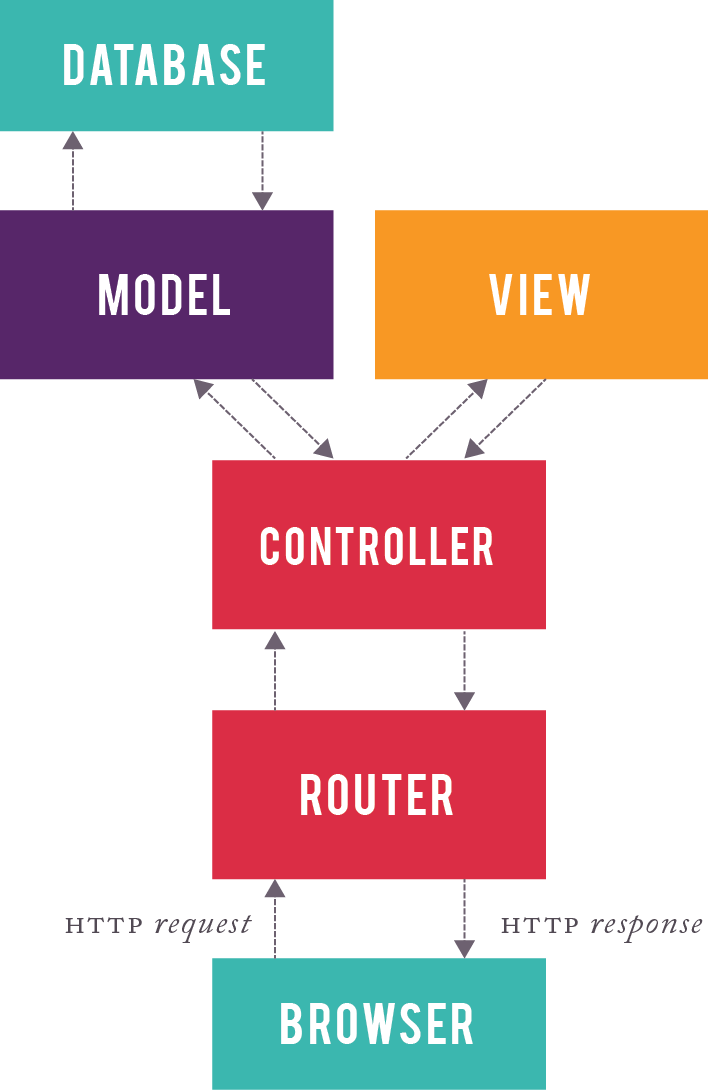
\includegraphics[width=0.5\hsize]{images/rails.png}
\caption{Html-reporter\label{RYS.1}}
\source{https://robots.thoughtbot.com/shared-terminology-yet-different-concepts-between-emberjs-and-rails}
\end{figure}

\subsection{Połączenie z bazą danych PostgreSQL}
\textit{PostgreSQL} jest SQL-ową bazą danych, rekomendowaną dla \textit{Ruby on Rails}, przez swoją ścisłą integrację z wcześniej wymienionym \textit{framework}em oraz posiada dobre narzędzia i metody zarządzania. Standardową bazą danych w aplikacjach stworzonych w \textit{Ruby on Rails} jest \textit{SQLite}, jednakże nie jest ona wspierana przez \textit{Heroku}, który jest najpopularniejszym darmowym serwer dla aplikacji w \textit{Ruby on Rails}. Brak wsparcia jest spowodowany tym, że \textit{SQLite} działa głównie w pamięci, i tylko od czasu do czasu zapisuje dane do pliku. O ile takie rozwiązanie jest dobre dla małych lokalnych aplikacji, których dane mogą być łatwo przenoszone, nie sprawdza się na serwerach \textit{Heroku}, gdyż w darmowej wersji, nasza aplikacja może działać maksymalnie przez 18 godzin na dobę po czym jest wyłączana. Takie nagłe wyłączenie spowodowałoby utratę całej bazy danych. Drugim ważnym aspektem jest skalowanie aplikacji. Większy program może zostać uruchomiony na większej ilości zasobów sprzętowych tak zwanych \textit{dyno}, a baza danych \textit{SQLite} może pracować tylko na jednym procesie, tak więc jeśli będzie więcej procesów każdy z nich będzie posiadać własną bazę danych a dane nie będą synchronizowane prawidłowo. W związku z powyższym powinniśmy używać \textit{PostgreSQL} na etapie produkcyjnym naszej aplikacji.\newline \indent Zmiana bazy danych z \textit{SQLite} na \textit{PostgreSQL} nie jest zbyt trudna. Pierwszym krokiem jest zainstalowanie bazy na komputerze, na którym ma być uruchomiona aplikacja. Na oficjalnej stronie można znaleźć linki do pobrania. Po zainstalowaniu, musimy dodać do naszej aplikacji \verb|gem 'pg'| który zapewnia kompatybilność z bazą \textit{PostgreSQL}, a usuwamy \verb|gem 'sqlite3'|. Następnie modyfikujemy plik \textit{database.yml}, który jest plikiem konfiguracyjnym naszej aplikacji. Ostatnim krokiem jest utworzenie bazy danych na nowym środowisku przy pomocy komendy \verb|rake db:create db:migrate|  
\subsection{Dodawanie gemów w Ruby on Rails}
Jedną z największych zalet Ruby on Rails jest dopasowanie się frameworka do naszych potrzeb za pomocą minibibliotek tzw. gemów, tworzonych przez developerów z całego świata.
W sieci można znaleźć tysiące różnych gemów, a każdy z nich posiada przeważnie tylko jedno specyficzne zadanie. Gemy, które są w ciągłym użytku są na bieżąco aktualizowane, dzięki czemu są poprawiane błędy i dodawane nowe funkcje. Przykładowo jeżeli chcemy testować naszą aplikacje, możemy to zrobić dzięki gemowi RSpec. Pozwala on na testowanie różnorakich elementów naszej aplikacji od walidacji pól w formularzach do kontrolerów i zapisywania danych w bazie.\newline \indent Aby dodać nowy gem do naszej aplikacji wystarczy dodać jego nazwę do pliku Gemfile w głównym katalogu naszej aplikacji go zapisać. Następnie wystarczy w terminalu otworzyć folder z naszą aplikacją i wpisać komendę "bundle install". Ruby on Rails automatycznie zainstaluje najnowszą wersję danego gemu, chyba, że wpisaliśmy konkretną wersję w pliku Gemfile. Całość przebiega szybko i sprawnie.

\subsection{Autoryzacja użytkowników}
Autoryzacja użytkowników jest jednym z najważniejszych zagadnień w aplikacji PicDrop. Dzięki niej logujemy się do aplikacji jak i do serwisów społecznościowych, na które chcemy umieścić zdjęcia. Bez niej ktoś obcy mógłby korzystać z naszych danych logowania z Facebooka i Flickr bez naszej wiedzy. Cały proces autoryzacji jest dość skomplikowany i przebiega w kilku etapach. Gdy chcemy się zalogować wpisujemy nasz login i hasło a następnie klikamy na guzik Log in. Nasz login jest adresem email i musi być unikatowy, dlatego mamy pewność, że nie będzie dwóch takich samych kont ale z różnymi hasłami, dzięki czemu nikt się nie zaloguje na nasze konto. \textit{Ember.js} pobiera dane z naszego formularza i wysyła je używając wiadomości \textit{JSON} do naszego serwera. Tam aplikacja generuje dla danego użytkownika klucz tzw. token, który jest przechowywany w bazie danych i na nim opiera się tzw. sesja dzięki, której jesteśmy zalogowani nawet jeśli odświeżymy stronę. Token jest odsyłany do \textit{Ember.js} i jesteśmy zalogowani. \newline \indent Jak pisałem we wcześniejszym rozdziale, aplikacja na serwerze posiada  trzy modele - \textit{User}, \textit{Photo} oraz \textit{Authorization}. Model \textit{User} jest zarządzany przez gem \textit{Devise}. Jest to najpopularniejszy gem do uwierzytelniania w Ruby on Rails. Ma wiele funkcji i składa się z 10 modułów dzięki czemu może być dostosowany do potrzeb developera. Wymienię tylko najważniejsze z nich dla mojej aplikacji. Pierwszy z nich to \textit{Database Authenticatable}, który szyfruje i zachowuje hasło w bazie danych to autoryzacji użytkownika podczas logowania. Drugi to \textit{Omniauthable} dodaje on wsparcie dla OmniAuth, który jest gemem do logowania się w aplikacjach \textit{Ruby on Rails} na różne serwisy społecznościowe. Omówię go dokładniej w następnym rozdziale. Następny to \textit{Timeoutable}, który porzuca sesję dla nieaktywnego użytkownika przez sprecyzowany okres czasu. Takie rozwiązanie znacznie zwiększa bezpieczeństwo naszych danych, ponieważ nawet jeśli zostawimy zalogowany komputer to po czasie wygaśnięcia sesji musimy się ponownie zalogować co nie pozwala użytkować naszego konta przez osoby trzecie.
\newline\indent \textit{Ember.js} do autoryzacji używa biblioteki \textit{Ember Simple Auth} i jej modułu kompatybilnego z \textit{Devise}, który nosi nazwę \textit{Ember Simple Auth Devise}. Biblioteka ta zapewnia kompleksowe zarządzanie sesją i logowaniem do aplikacji opartych na \textit{Ember.js}, gdyż posiada wiele modułów dla różnych typów uwierzytelniania. Są to między innymi \textit{simple-auth-oauth2 }, który pozwala na logowanie w standardzie \textit{OAuth2}. Standard ten jest używany przez Facebooka i zostanie dokładniej omówiony w jednym z kolejnych rozdziałów. Kolejny moduł to \textit{simple-auth-torii}. Jest to moduł kompatybilny z biblioteką \textit{Torii}, która odpowiada za logowanie w standardzie \textit{OAuth 1a}. Standard ten jest wykorzystywany między innymi przez \textit{Twittera} i \textit{Flickra}.

\subsection{Połączenie z API różnych sieci społecznościowych} l User Authorization URL: Access Token URL: wysyłanie zdjęc
\textit{API} aplikacji łączy się z różnymi sieciami społecznościowymi przez gem \textit{Omniauth}. Dzięki niemu możemy po zalogowaniu, wysyłać nasze zdjęcia na dwa serwisy jednocześnie. W zależności od serwisu społecznościowego, używany jest inny standard protokółu \textit{OAuth}. Pierwszym z nich jest \textit{OAuth 1.0a}, używany przez \textit{Twittera} i \textit{Flickr}a. Jest on starszym i bardziej skomplikowanym standardem logowania. Logownie przebiega w 3 krokach. Pierwszy krok to wysłanie prośby o tak zwany \textit{Request Token}, który zawiera \textit{request oauth token} oraz \textit{request oauth secret} a nasze zapytanie wysyła m. in.  identyfikator i sekretny kod naszej aplikacji oraz datę i czas zapytania. Wygląda mniej więcej tak:
\begin{minted}[frame=single, fontsize=\normalsize, breaklines=true]{ruby}
https://www.flickr.com/services/oauth/request_token
?oauth_nonce=89601180
&oauth_timestamp=1305583298
&oauth_consumer_key=653e7a6ecc1d528c516cc8f92cf98611
&oauth_signature_method=HMAC-SHA1
&oauth_version=1.0
&oauth_callback=http%3A%2F%2Fwww.example.com
\end{minted}
\newpage
 Gdy prośba zostaje przetworzona, serwer odsyła \textit{Request Token} 
\begin{minted}[frame=single, fontsize=\normalsize, breaklines=true]{ruby}
 oauth_callback_confirmed=true
&oauth_token=72157626737672178-022bbd2f4c2f3432
&oauth_token_secret=fccb68c4e6103197
\end{minted}
Następnie użytkownik zostaje przekierowany do strony logowania gdzie podaje swoje dane. Po poprawnym zalogowaniu serwer odsyła \textit{oauth verifier}.
\begin{minted}[frame=single, fontsize=\normalsize, breaklines=true]{ruby}
http://www.example.com/
?oauth_token=72157626737672178-022bbd2f4c2f3432
&oauth_verifier=5d1b96a26b494074
\end{minted}
 Ostatnim krokiem jest wysłanie przez naszą aplikację \textit{Request Tokena} oraz \textit{Oauth verifiera} do serwerów autoryzacji w celu uzyskania \textit{Access Tokena} dzięki któremu możemy się zalogować.
 \begin{minted}[frame=single, fontsize=\normalsize, breaklines=true]{ruby}
 https://www.flickr.com/services/oauth/access_token
?oauth_nonce=37026218
&oauth_timestamp=1305586309
&oauth_verifier=5d1b96a26b494074
&oauth_consumer_key=653e7a6ecc1d528c516cc8f92cf98611
&oauth_signature_method=HMAC-SHA1
&oauth_version=1.0
&oauth_token=72157626737672178-022bbd2f4c2f3432
&oauth_signature=UD9TGXzrvLIb0Ar5ynqvzatM58U%3D
\end{minted}
\newpage\indent W standardzie OAuth 2.0, używany przez między innymi \textit{Facebooka}. Gdy chcemy się zalogować do tego serwisu wystarczy nacisnąć guzik logowania, który przekierowuje nas do adresu naszego API tj. \verb|/users/auth/facebook|. Następnie \textit{Omniauth} łączy się z serwerami \textit{Facebook'a} generując mniej więcej taki adres 
\begin{minted}[frame=single, fontsize=\normalsize, breaklines=true]{ruby}
https://www.facebook.com/auth?response_type=code
&client_id=CLIENT_ID&redirect_uri=REDIRECT_URI&scope=photos
\end{minted}
 W nim znajduje się prośba o kod autoryzacyjny, identyfikator naszej aplikacji, adres do przekierowania po wpisaniu prawidłowych danych z \textit{Facebook'a} oraz uprawnienia aplikacji, na które użytkownik musi zezwolić, żeby się zalogować. Po podaniu prawidłowych danych zostaje odesłany kod autoryzacyjny, który zostaje zamieniony przez \textit{Omniauth }na tak zwany \textit{Access Token} a użytkownik zostaje zalogowany do aplikacji. Aby użytkownicy mogli się logować do naszej aplikacji należy wcześniej ją zarejestrować na stronach dla \textit{web developer}ów \textit{Facebooka} oraz \textit{Flickr}a. Tam podając dane nasze oraz aplikacji zostaje wygenerowany identyfikator. Wpisujemy go w piliku konfiguracyjnym \textit{Omniuth}, aby serwisy wiedziały jaka aplikacja chce się zalogować.

\section{Front-end aplikacji}

\subsection{Budowa Front-endu w oparciu o framework EmberJS }
Warstwa wizualna aplikacji czyli tak zwany front-end został wykonany przy użyciu frameworka EmberJS. Dzięki temu łatwiej zarządzać tą cześcią aplikacji. \textit{EmberJS} opiera się na wzorcu \textit{Model-View-Controler} \footnote{ang. Model-Widok-Kontroler} co oznacza, że składa się z
trzech podstawowych części odpowiedzialnych za różne akcje. 
\begin{figure}[H]
\centering
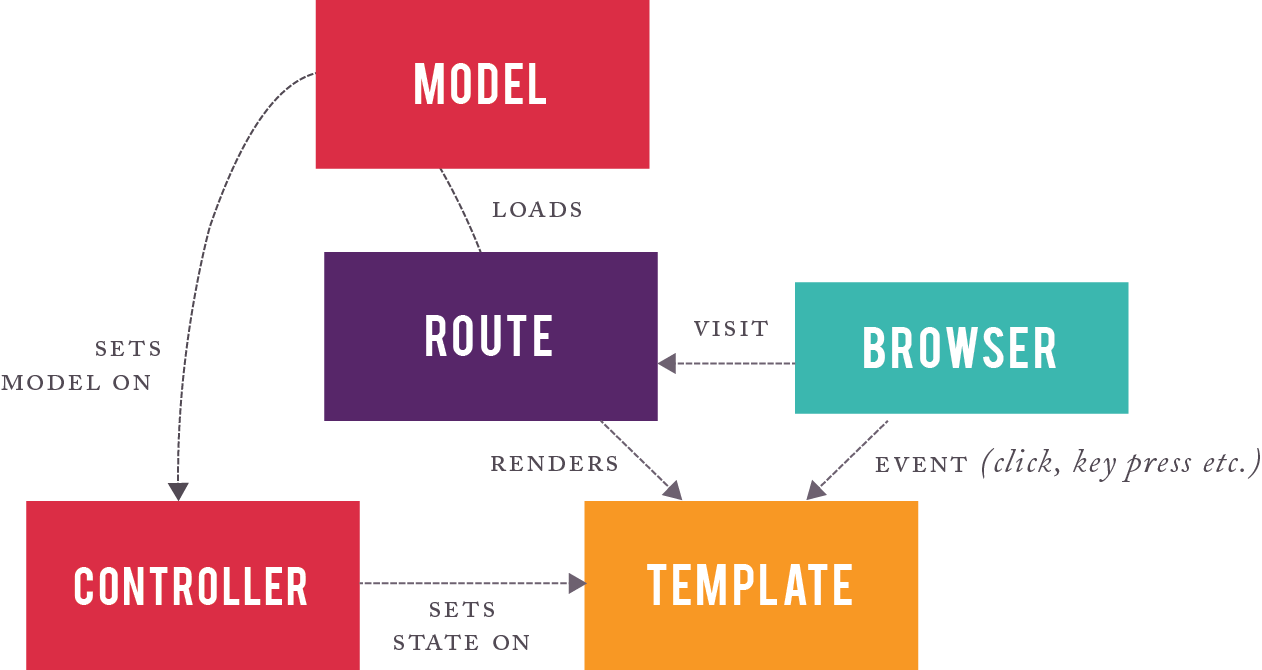
\includegraphics[width=0.7\hsize]{images/ember.png}
\caption{Diagram budowy Ember.js\label{RYS.1}}
\source{https://robots.thoughtbot.com/shared-terminology-yet-different-concepts-between-emberjs-and-rails}
\end{figure}
Model  jest pewną reprezentacją problemu bądź logiki aplikacji. W naszym przypadku model jest szablonem z opisanymi typami danych danego zasobu np. zdjęcia. Model również komunikuje się z Ember Data czyli warstwą aplikacji bezpośrednio komunikującą się z serwerem.  Widok opisuje, jak wyświetlić pewną część modelu w ramach interfejsu użytkownika. W EmberJS widok składa się z tak zwanych templates czyli kodem HTML z aktywnie zmieniającymi się częściami. Kontroller przyjmuje dane wejściowe od użytkownika i reaguje na jego akcje, zarządzając aktualizacje modelu oraz odświeżenie widoków. Kontroler w EmberJS pobiera dane z modelu oraz zarządza akcjami w widoku.

\subsection{Połączenie z API}
Połączenie z serwerem aplikacji jest jedną z najważniejszych rzeczy w całej aplikacji. To dzięki niemu możemy się komunikować z serwerem oraz przetwarzac dane z bazy danych. EmberJS do pobierania i przetwarzania danych korzysta z biblioteki Ember Data. Ma ona kilka wbudowanych tzw. adapterów do połączenia z różnymi typami serwerów napisanych w różnych językach i technologiach. W mojej aplikacji używam ActiveModelAdapter, który działa bezproblemowo z ActiveModel w Ruby on Rails przeprowadzając serializacje i deserializację danych z EmberJS do wiadomości JSON.

\subsection{Opis narzędzia Ember-CLI}
Ember-CLI (Command Line Interface) to program narzędziowy, który zarządza aplikacją napisaną we frameworku EmberJS. Głównymi zaletami korzystania z tego narzędzia jest zarządzanie plikami, zależnościami, proste dodawanie wtyczek, uruchamianie serwera, generowanie konkretnych części programu jak np. model lub kontroler.

\subsection{Dodawanie wtyczek do aplikacji w EmberJS}
Wtyczki są to programy dodające jakąś funkcjonalność do naszego programu, dzięki czemu nie musimy wszystkich elementów pisać od podstaw. Wystarczy jak poszukamy wtyczki zapewniającej nam funkcjonalność, której szukamy np. t17-ember-upload pozwala na wgrywanie zdjęć do naszej aplikacji poprzez proste \textit{Drag \& Drop}\footnote{pol. Przeciągnij i upuść}.  Aby dodać wtyczkę wystarczy zainstalować ją przy użyciu NPM lub bowera  po czym dodać app.import w pliku Brocfile.js. Następnie należy zaimportować konkretny moduł z wtyczki do naszej części aplikacji i już można używac widoku oraz akcji z wtyczki.
\subsection{Same origin policy oraz Cross-origin resource sharing} 
\textit{Same Origin Policy} uniemożliwia dwóm osobnym kontekstom Javascript modyfikacji swoich drzew DOM. Dzięki temu strona Agresora aggressive.com nie może modyfikować DOM strony Banku bank.com, w sytuacji kiedy np. te dwie strony są otwarte w kartach przeglądarki. Jednakże jeśli chcemy aby skrypt z jednego kontekstu modyfikowały inny takie zmiany zostaną wykonane. Wszystko dlatego, że strona ma ten sam \textit{Origin} czyli pochodznie. Na pochodzenie ma wpływ:
\begin{itemize}
\item protokół
\item host
\item port
\end{itemize}
Zasada \textit{SOP} jest jednocześnie zbawieniem i przekleństwem. Z jednej strony, jest to mechanizm skutecznie chroniący każdą stronę internetową, z drugiej – ogranicza developerów, którzy chcą np. asynchronicznie pobrać zasób z innej domeny. Aby pomóc developerom firma W3C wprowadziła \textit{Cross-Origin Resource Sharing} \footnote{and. dzielenie zasobów różnego pochodzenia}. Jest to metoda omijania SOP polegająca na odpowiednim ustawianiu nagłówków HTTP. Przeglądarka wysyła do serwera nagłówek “Origin”. Mówi w nim z jakiej strony chcemy się dostać do zasobu. Serwer musi zgodzić się na stronę źródłową. Załóżmy, że strona jest pod adresem http://moja-strona.pl a API ma adres http://moje-api.pl/api. Żądanie przeglądarki będzie wyglądać tak:
\begin{minted}[frame=single, fontsize=\normalsize, breaklines=true]{ruby}
GET /api HTTP/1.1
Origin: http://moja-strona.pl
Host: moje-api.pl
Accept-Language: en-US
User-Agent: Mozilla/5.0
\end{minted}
Odpowiedź serwera to:
\begin{minted}[frame=single, fontsize=\normalsize, breaklines=true]{ruby}
Access-Control-Allow-Origin: http://moja-strona.pl
Content-Type: text/html; charset=utf-8
\end{minted}
Nagłówek Access-Control-Allow-Origin mówi przeglądarce, że serwer zgadza się, żeby moja-strona.pl sięgała do naszego API. Można w tym miejscu ustawić gwiazdkę, wtedy serwer zgadza się na wszystkie strony.Aby móc wykorzystywać Cross-Origin Resource Sharing w swoim serwisie muszą zostać spełnione dwa  warunki:
\begin{itemize}
\item przeglądarka musi obsługiwać CORS
\item serwer, do którego się odwołujemy musi być odpowiednio skonfigurowany
\end{itemize}
 Wszystkie obecne przeglądarki obsługują \textit{CORS} także punkt pierwszy nie jest problemem. Natomiast konfiguracja serwera czyli naszego \textit{API} przebiega następująco. Po pierwsze musimy zainstalować \verb|gem 'rack-cors'|, następnie dodajemy następujący kod do pliku \verb|application.rb|
\begin{minted}[frame=single, fontsize=\normalsize, breaklines=true]{ruby}
config.middleware.use Rack::Cors do
   allow do
       origins "*"
       resource "*", headers: :any, methods: [:get, :post, :put, :delete, :options]
   end
end
\end{minted}
Po ponownym uruchomieniu serwera jest on odpowiednio skonfigurowany.
\newline\indent W \textit{Ember.js} nie potrzebujemy dodawać nowych modułów, wystarczy dodać do pliku \verb|enviroment.js| kod:
\begin{minted}[frame=single, fontsize=\normalsize, breaklines=true]{js}
ENV.contentSecurityPolicy = {
    'default-src': "http://www.facebook.com/",
    'script-src': "'self' 'unsafe-inline' 'unsafe-eval' ",
    'font-src': "'self' http://fonts.gstatic.com", 
    'connect-src': "'self' http://localhost:3000/ http://localhost:3000/photos http://127.0.0.1:3000 http://localhost:3000/users/sign_in ",
    'img-src': "'self' http://localhost:3000 http://localhost:4200/category" ,
    'report-uri':"'localhost'",
    'style-src': "'self' 'unsafe-inline' http://fonts.googleapis.com", 
    'media-src': "'self'"
  }
\end{minted}
\chapter{Testy}
\section{Testowanie API przy użyciu RSpec}
\textit{RSpec} jest najpopularniejszą biblioteką używaną do testowania aplikacji napisanych w \textit{Ruby on Rails}. Testy dzielą się na 3 typy. Pierwszy z nich to testy kontrolera, które spawdzają poprawność zapisywania i odczytywania danych w bazie. Dzięki temu wiadomo czy aplikacja prawidłowo komunikuje się z bazą danych. Drugi typ testów to testy modelu danych. Testy te głównie sprawdzają czy walidatory, czyli elementy sprawdzające poprawność i format danych wpisywanych przez użytkownika, działają prawidłowo. Gdyby nie było walidacji, można by było na przykład zamiast imienia wpisać dowolny ciąg znaków o dowolnej długości co może powodować konflikty i błędy podczas przetwarzania danych. Trzeci typ testów to testy funkcjonalne, czyli testy zachowania interfejsu użytkownika na konkretne akcje, jak na przykład wpisanie w pole formularza lub kliknięcie na guzik. Do testów funkcjonalnych często używana jest dodatkowa biblioteka \textit{Capybara}, która współpracuje z Rspec. 

\subsection{Raport z testów API}
W \textit{API} aplikacji zostało przetestowane głównie łączenie się aplikacji ze sieciami społecznościowymi tj. \textit{Facebook} oraz \textit{Flickr}. 
\section{Testowanie Front-end przy użyciu QUnit}
\textit{QUnit} jest standardową biblioteką używaną do testowania aplikacji napisanych w \textit{Ember.js}. Pozwala na pisanie zarówno \textit{Unit tests} \footnote{ang. Testy jednostkowe} jak i \textit{Acceptance tests} \footnote{ang. Testy akceptujące}.  Testy jednostkowe to wyizolowane części funkcjonalności, bez ich zależności od innych elementów. Przykładowo:
\begin{itemize}
\item Użytkownik ma imię.
\item Użytkownik ma imię i nazwisko, które nie może przekaraczać 50 znaków.
\item Zdjęcie ma nazwę.
\end{itemize}
Testy akceptacyjne są używane do testowania interakcji użytkownika z aplikacją. Przykładowo:
\begin{itemize}
\item Użytkownik jest w stanie zalogować się przez formularz logowania.
\item Użytkownik może utworzyć nowe konto.
\item Użytkownik po zalogowaniu jest przekierowany do strony głównej.
\end{itemize}
Uruchamianie testów może przebiegać na dwa sposoby. Pierwszy z nich to wpisanie komendy \verb|ember test|. Aplikacja uruchomi wszystkie testy w konsoli i ewentualne błędy zostaną również tam wyświetlone. Drugim sposobem jest normalne uruchomienie serwera i wpisanie adresu serwera z koncówką \verb|/tests|. W oknie przeglądarki zostaną pokazane wszystkie testy.
\newline \indent Warto wspomnieć również o tzw. \textit{helperach} czyli plikach zawierających niestandardowe metody pomagające testować kod.
\subsection{Raport z testów Front-end}
W \textit{front-endzie} główny nacisk został położony na przetestowanie logowania i uwierzytelniania użytkowników i te elementy zostały przetestowane automatycznie. Reszta aplikacji została przetestowana ręcznie a znalezione błędy zostały usunięte.
\chapter{Wkład własny}
% zakończenie
\summary
W niniejszej pracy starałem się pokazać budowę aplikacji modularnej, zalety i wady takiego rozwiązania oraz szereg różnych problemów z jakimi musi się uporać developer podczas pisania takowej aplikacji. 
% załączniki (opcjonalnie):
\appendix
\chapter{Tytuł załącznika jeden}

Treść załącznika jeden.
\chapter{Tytuł załącznika dwa}

Treść załącznika dwa.

% literatura (obowiązkowo):
\bibliographystyle{unsrt}
\bibliography{mgr}

\nocite {magiaUI}
\nocite {design}
\nocite {projektowanieUI}
\nocite {StiveKrug}
\nocite{DouglasCrockford}
\nocite {UIRails}
\nocite {modelingUI}
\nocite {rspecDoc}
\nocite {railsDoc}
\nocite {emberDoc}
\nocite{emberCLIDoc}
\nocite{emberRails}
\nocite{emberTutorial}
\nocite{emberIntro}

% spis tabel (jeżeli jest potrzebny):
\listoftables

% spis rysunków (jeżeli jest potrzebny):
\listoffigures

\oswiadczenie

\end{document}
